%
% File acl2015.tex
%
% Contact: car@ir.hit.edu.cn, gdzhou@suda.edu.cn
%%
%% Based on the style files for ACL-2014, which were, in turn,
%% Based on the style files for ACL-2013, which were, in turn,
%% Based on the style files for ACL-2012, which were, in turn,
%% based on the style files for ACL-2011, which were, in turn, 
%% based on the style files for ACL-2010, which were, in turn, 
%% based on the style files for ACL-IJCNLP-2009, which were, in turn,
%% based on the style files for EACL-2009 and IJCNLP-2008...

%% Based on the style files for EACL 2006 by 
%%e.agirre@ehu.es or Sergi.Balari@uab.es
%% and that of ACL 08 by Joakim Nivre and Noah Smith

\documentclass[11pt]{article}
\usepackage{acl2015}
\usepackage{times}
%\usepackage{url}
\usepackage{latexsym}
\usepackage{algorithm}
\usepackage{algorithmic}
\usepackage{fullpage}
\usepackage{graphicx}
\usepackage{longtable}
\usepackage{lscape}
\usepackage{CJKutf8}
\usepackage[hyphens]{url}
\usepackage[labelfont=bf, textfont=bf]{caption}
%\begin{CJK*}{UTF8}{gbsn}
%\setlength\titlebox{5cm}

% You can expand the titlebox if you need extra space
% to show all the authors. Please do not make the titlebox
% smaller than 5cm (the original size); we will check this
% in the camera-ready version and ask you to change it back.

% Tao: All upper-case is hard to read.
%\title{LEARNING SECOND LANGUAGE FROM NEWS WEBSITES}
\title{Interactive Second Language Learning from News Websites}

%\author{First Author \\
%  Affiliation / Address line 1 \\
%  Affiliation / Address line 2 \\
%  Affiliation / Address line 3 \\
%  {\tt email@domain} \\\And
%  Second Author \\
%  Affiliation / Address line 1 \\
%  Affiliation / Address line 2 \\
%  Affiliation / Address line 3 \\
%  {\tt email@domain} \\}

\date{}

\begin{document}

\maketitle
\begin{abstract}
%Learning a second language is difficult
%and requires constant revision and immersion.
%Fortunately, many of us read news
%online everyday. In this paper, we propose
%a web browser extension that allows
%a reader to learn a second language vocabulary
%while reading news online. We hypothesize
%Since we find a word’s context to be useful
%in learning a vocabulary, we further
%use word sense disambiguation (WSD) to
%show the best translation for each word in
%the context. Our proposed WSD method,
%leveraging the extension of standard machine
%translation system, significantly betters
%baseline methods in both coverage
%and accuracy. We also elaborate on
%the issues of determining appropriate distractors
%for multiple-choice word mastery
%quizzes .
%We conducted a user survey to evaluate
%our system against user requirements collected
%through an earlier survey.


We propose a web browser extension that allows readers to learn a
second language vocabulary while reading news online.  Injected
tooltips allow readers to look up selected vocabulary and give
interactive tests to assess vocabulary mastery.  

We discover that two key system components needed improvement, both
which stem from the need to model context.  These two issues are in
practical word sense disambigution (WSD) to aid translation quality
and constructing the interactive tests. We start with Microsoft's Bing
translation API but employ additional dictionary based heuristics that
significantly improve translation quality over a baseline in both
coverage and accuracy. We also propose techniques for generating
appropriate distractors for multiple-choice word mastery tests.  Our
preliminary user survey confirms the need and viability of such a
language learning platform.

\end{abstract}

% Tao: Need to highlight the research gap (e.g., the drawbacks of existing methods for CWSD) and contributions of this work
\section{Introduction}
\label{intro}

%
% The following footnote without marker is needed for the camera-ready
% version of the paper.
% Comment out the instructions (first text) and uncomment the 8 lines
% under "final paper" for your variant of English.
% 
\iffalse
\blfootnote{
    %
    % for review submission
    %
    \hspace{-0.65cm}  % space normally used by the marker
    Place licence statement here for the camera-ready version, see
    Section~\ref{licence} of the instructions for preparing a
    manuscript.
    %
    % % final paper: en-uk version (to license, a licence)
    %
    % \hspace{-0.65cm}  % space normally used by the marker
    % This work is licensed under a Creative Commons 
    % Attribution 4.0 International Licence.
    % Licence details:
    % \url{http://creativecommons.org/licenses/by/4.0/}
    % 
    % % final paper: en-us version (to licence, a license)
    %
    % \hspace{-0.65cm}  % space normally used by the marker
    % This work is licenced under a Creative Commons 
    % Attribution 4.0 International License.
    % License details:
    % \url{http://creativecommons.org/licenses/by/4.0/}
}
\fi

%Formally learning a new language is time-consuming and requires learners to invest a significant
%amount of effort. A Chrome Extension, {\it WordNews}, was developed by \cite{tao2014} to allow users to pick up Chinese vocabulary while reading online news articles. WordNews makes language learning efficient and attractive by interleaving language
%learning with the daily activity of online news reading. 
%WordNews allows users to learn from real-world examples, and to learn words in context, which is required for effective learning of vocabulary \cite{Hirsch03readingcomprehension}.

% Tao: The logic of this section does flow well: 1) some paragraphs have duplicate information, and 2) the motivation and contribution of this paper is not clear. I prefer to move the literature review to a separate section since it is quite long (almost 1.5 pages).
% Tao: tried to edit (partial)

A word takes on different meanings, largely dependent on the context
in which it is used. For example, the word ``bank'' could mean ``slope
beside a body of water'', or a ``depository financial
institution''~\footnote{\url{http://wordnetweb.princeton.edu/perl/webwn?s=bank}}. Word
Sense Disambiguation (WSD) is the task of identifying the contextually
appropriate meaning of the word. WSD is often considered a
classification task, in which the classifier predicts the sense from a
possible set of senses, known as a sense inventory, given the target
word and the contextual information of the target word. Existing WSD
systems can be categorised into either data-driven supervised or
knowledge-rich approaches. Both approaches are considered to be
complementary to each other.

%The task of Word Sense Disambiguation (WSD) is the task of identifying the correct sense/meaning of a word out of possible senses defined in a sense inventory. 
Word embeddings have become a popular word representation formalism,
and many tasks can be done using word embeddings. The effectiveness of
using word embeddings has been shown in
% Tao: cite a few more papers
several NLP tasks \cite{Turian10wordrepresentations}. The goal of our
work is to apply and comprehensively compare different uses of word
embeddings, solely with respect to WSD. We perform evaluation of the
effectiveness of word embeddings on monolingual WSD tasks from
Senseval-2 (held in 2001), Senseval-3 (held in 2004), and
SemEval-2007. After which, we evaluate our approach on English--Chinese
Cross-Lingual WSD using a dataset that we constructed for %the use of
evaluating our approach on the translation task used in educational
applications for language learning. %, such as {\it  MindTheWord}{\footnote{\url{https://chrome.google.com/webstore/detail/mindtheword/fabjlaokbhaoehejcoblhahcekmogbom?hl=en}}} and {\it WordNews}~\cite{tao2014}.

%% Min: Nav too ordinary, try without it.
% The structure of this paper will be as follows: we have first reviewed related work and methods regarding WSD, next we will discuss the applications of WSD to a category of educational applications, and outlining possible future work finally in the conclusion. 

%The task of Word Sense Disambiguation (WSD) is the task of identifying the correct sense/meaning of a word out of possible senses defined in a sense inventory. Word embeddings is a popular technique in NLP in recent years, and many tasks can be done using 
%word embeddings. The effectiveness of
%using word embeddings has been shown in 
%% Tao: cite a few more papers
%several NLP tasks \cite{Turian10wordrepresentations}
%The goal of this work is to apply and compare different uses of word embeddings for WSD. We perform evaluation of the effectiveness of word embeddings on monolingual WSD tasks from Senseval-2 (held in 2001), Senseval-3 (held in 2004), and SemEval-2007. After which, we evaluate our approach on 
%English-Chinese Cross-Lingual WSD using a dataset that we constructed for the use of evaluating our approach on the translation task used in educational applications for language learning, such as MindTheWord {\footnote{\url{https://chrome.google.com/webstore/detail/mindtheword/fabjlaokbhaoehejcoblhahcekmogbom?hl=en}}} and WordNews.
%
%
%
%A word can have different meanings depending on the context in which it is used. For example, the word ``bank" could mean ``slope beside a body of water", or a ``depository financial institution"~\footnote{\url{http://wordnetweb.princeton.edu/perl/webwn?s=bank}}. Word Sense Disambiguation is the task of identifying the contextually appropriate meaning of the word. Word Sense Disambiguation can be considered a classification task, in which the classifier predicts the sense from a possible set of senses, known as a sense inventory, given the target word and the contextual information of the target word. Existing WSD systems can be categorised into either supervised or knowledge-rich approaches. Both approaches are considered to be complementary to each other. 
%
%
%Word Sense Disambiguation is a well-studied problem and there are many different methods. Existing methods can be broadly categorised into supervised approaches, where machine learning techniques are used to learn from labeled training data, and unsupervised knowledge-rich techniques, which do not rely on labeled data. Unsupervised techniques are knowledge-rich, and rely heavily on knowledge bases and thesaurus, such as WordNet. It is noted by Navigli \shortcite{Navigli09wordsense} that supervised approaches using memory-based learning and SVM approaches have worked best. 
%%For these approaches, it is common that the only knowledge used is the first sense in WordNet, which is used as a fallback if the system is unable to disambiguate the word in the test data. 
%
%Supervised approaches involve the extraction of features and then classification using machine learning. \shortcite{Zhong2010} developed an open-source WSD system, IMS, which was state-of-the-art at the time it was developed. It is a supervised-learning based WSD system, which first has to be trained using a set of training data. IMS uses three feature types, 1. individual words in the context surrounding the target word, 2. specific ordered sequences of words appearing at specified offsets from the target word, 3. Part-Of-Speech tags of the surrounding 3 words.
%
%% \begin{itemize}
%
%% 	\item  Surrounding Words\\
%% 	Surrounding words include individual words in the surrounding context. Sentence boundaries can be crossed in this feature. Stopwords, punctuation, character symbols, and numbers are discarded. 
%
%% 	\item Local Collocations\\
%% 	A collocation is an ordered sequence of words appearing in a specified offset from the target word. 11 location collocation features are used. They are $C_{-2},_{-2}$, $C_{-1},_{-1}$,
%% 	$C_{1},_{1}$, $C_{2},_{2}$, $C_{-2},_{-1}$, $C_{-1},_{1}$, $C_{1},_{2}$, $C_{-3},_{-1}$,
%% 	$C_{-2},_{1}$, $C_{-1},_{2}$, and $C_{1},_{3}$. $C_{i},_{j}$ refers to the ordered sequence of words between positions $i$ and $j$ relative to the target word. 
%
%% 	\item Part-Of-Speech (POS) tags of surrounding words\\
%% 	The POS tags of the three words to the left and right of the target word are used for disambiguation. If a word in the window is not in the same sentence, its POS tag will be assigned as null. %The default POS tagger in the OpenNLP toolkit~\footnote{\url{http://opennlp.apache.org/}} is used.
%% \end{itemize} 
%
%Each of the features are binary features, and IMS trains a model for each word. IMS then uses an SVM for classification. IMS is open-source, provides state-of-the-art performance at the time of its publication, and is easy to extend. As such, our proposed approach focuses heavily on IMS. 
%
%Training data is required to train IMS, which is a supervised system. 
%An example of training data for training WSD system is the One-Million Sense-Tagged Instances \cite{taghipour2015one}. This is the largest dataset we know of for training WSD systems, and we make use of it for training our systems for the All-Words tasks. 
%
%WSD systems can be evaluated using either fine-grained scoring or coarse-grained scoring. In fine-grained scoring, every sense is equally distinct from each other, and answers must exactly match. In coarse-grained scoring, similar senses are grouped and treated as a single sense. A main bottleneck to Word Sense Disambiguation is the granularity of senses. Since word senses are subjective, and the boundaries between each sense is not always well-defined, an important measure for any task is the inter-annotator agreement. The inter-annotator agreement is considered the upper bound of a task. 
%
%A problem of Word Sense Disambiguation is that the granularity of senses are subjective and may not be well-defined. WordNet is a fine-grained resource, and even human annotators have trouble distinguishing between different senses of a word \cite{edmonds2002introduction}. 
%%In some WSD tasks during Senseval, coarse-grained scoring was done in order to deal with this problem. In these evaluations, similar senses of a word are clustered together and are considered to be the same sense. 
%
%Cross-Lingual WSD was partially conceived as a further attempt to solve this issue. In Cross-Lingual WSD, the specificity of a sense is determined by its correct translation. The sense inventory is the possible translations of each word in another language. Two instances are said to have the same sense if they map to the same translation in that language. In SemEval-2010~\footnote{\url{http://stel.ub.edu/semeval2010-coref/}}, a task for Cross-Lingual WSD was introduced. SemEval-2013~\footnote{\url{https://www.cs.york.ac.uk/semeval-2013/}} featured the second iteration of this task. These tasks were tasks in which an English noun were the targeted words, and the word senses were the translations in Dutch, French, Italian, Spanish and German. 
%
%
%Traditional WSD approaches are used in Cross-Lingual WSD, although some approaches make use of Statistical Machine Translation methods and features from translation. Cross-Lingual WSD involves training by making use of parallel or multilingual corpora. In the Cross-Lingual WSD task in SemEval-2013, the top approaches used a classification approach or a statistical machine translation approach. 
%
%In NLP, words can be represented in a vector space model. Traditionally, this has been done with {\it one-hot} binary vectors, where there is only one non-zero value in a high-dimensional vector. In this encoding, each dimension represents the presence of a word, and the number of dimensions of the vector space is the size of the vocabulary. In one-hot encoding, all words are considered to be independent of each other. A problem with one-hot encoding is that the large number of dimensions makes machine learning vulnerable to over-fitting. There is no notion of word similarity and all words are independent of each other. A distributed representation of words, such as word embeddings, resolves these problems by encoding words into a low dimensional space. In word embeddings, information about a word is distributed across multiple dimensions, and similar words are expected to be close to each other. Examples of word embeddings are Continuous Bag of Words \cite{mikolovword2vec}, Collobert \& Weston's Embeddings \cite{collobert2008unified}, and GLoVe \cite{pennington2014glove}. We implemented and evaluated the use of word embedding features using these embeddings in IMS. 
%
%
%An unsupervised approach using word embeddings for WSD is described by Chen \shortcite{chen2014}. This uses a model for finding representation of senses, rather than just for words, initialised using WordNet's glosses of senses. These sense vectors can then be used during Word Sense Disambiguation. A context vector can be computed by taking the average of the words in a sentence. For disambiguating a single word, the sense with the sense vector that gives maximum Cosine Similarity with this context vector is chosen as the result for disambiguation. Chen {\it et al.} gives an algorithm to disambiguate words starting from the words with fewer senses first. 
%
%A different approach is to work on extending existing WSD systems. Turian \shortcite{Turian10wordrepresentations} suggests that for any existing supervised NLP system, a general way of improving accuracy would be to use unsupervised word representations as additional features. Taghipour \shortcite{Taghipour15} used C\&W embeddings as a starting point and implemented word embeddings as a feature type in IMS. For a specified window, vectors for the surrounding words in the windows, excluding the target word, are obtained from the embeddings and are concatenated, producing $d * (w-1)$ features, where $d$ is the number of dimensions of the vector, and w is the window size. Each feature is a floating point number, which is the value of the vector in a dimension. We note that \cite{Taghipour15} only reported results for C\&W embeddings, and did not experiment on other types of word embeddings.  
%
%Other supervised approaches using word embeddings include AutoExtend \cite{rothe2015autoextend}, which extended word embeddings to create embeddings for synsets and lexemes. In their work, they also extended IMS, but used their own embeddings. Three feature types were introduced by this work, which has some similarities to how Taghipour used word embeddings, but without Taghipour's method of scaling each dimension of the word embeddings. \\
%
%
%% Apart from reviewing work on WSD, we can generalise WSD as a classification problem and look at other approaches to perform classification. We therefore experiment with the approach of using a Neural Network for classification. In Natural Language Processing, much work has been done with Recursive Neural Networks, such as Recurrent Neural Networks, and Recursive Autoencoders. These networks have shown extremely promising results in many NLP classification tasks, such as Sentiment Classification, obtaining state-of-the-art results. 
%
%The structure of this paper will be as follows: we have first reviewed related work and methods regarding WSD, next we will discuss the applications of WSD to a category of educational applications, and outlining possible future work finally in the conclusion. 




% Tao: Temporarily put the 3-in-1 screenshot here. Please move it to the proper place.
%% \begin{figure*}[ht]
%% \centering
%%     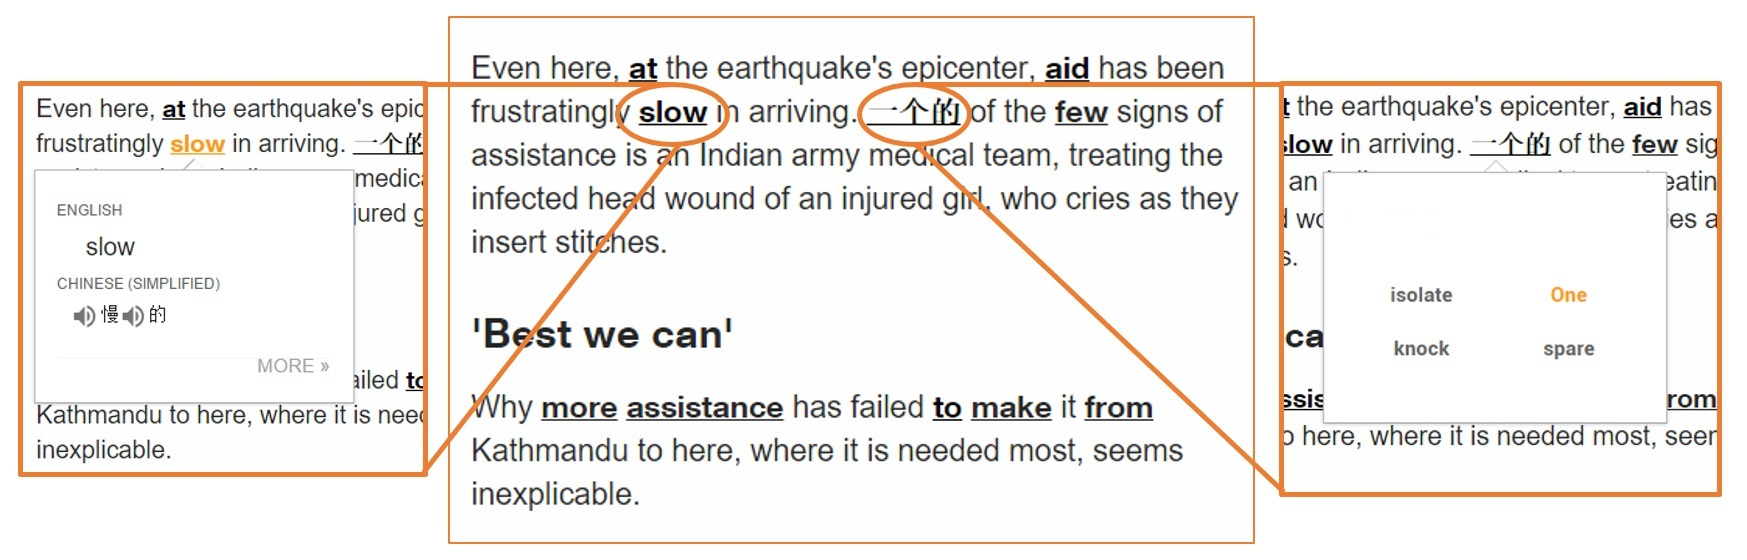
\includegraphics[width=0.99\textwidth]{chrome_extension.jpg}
%% 	\caption{............}
%% 	\label{fig:chrome_extension_1}
%% \end{figure*}

% Tao: Temporarily put the 3-in-1 screenshot here. Please move it to the proper place.
\begin{figure*}[ht]
\centering
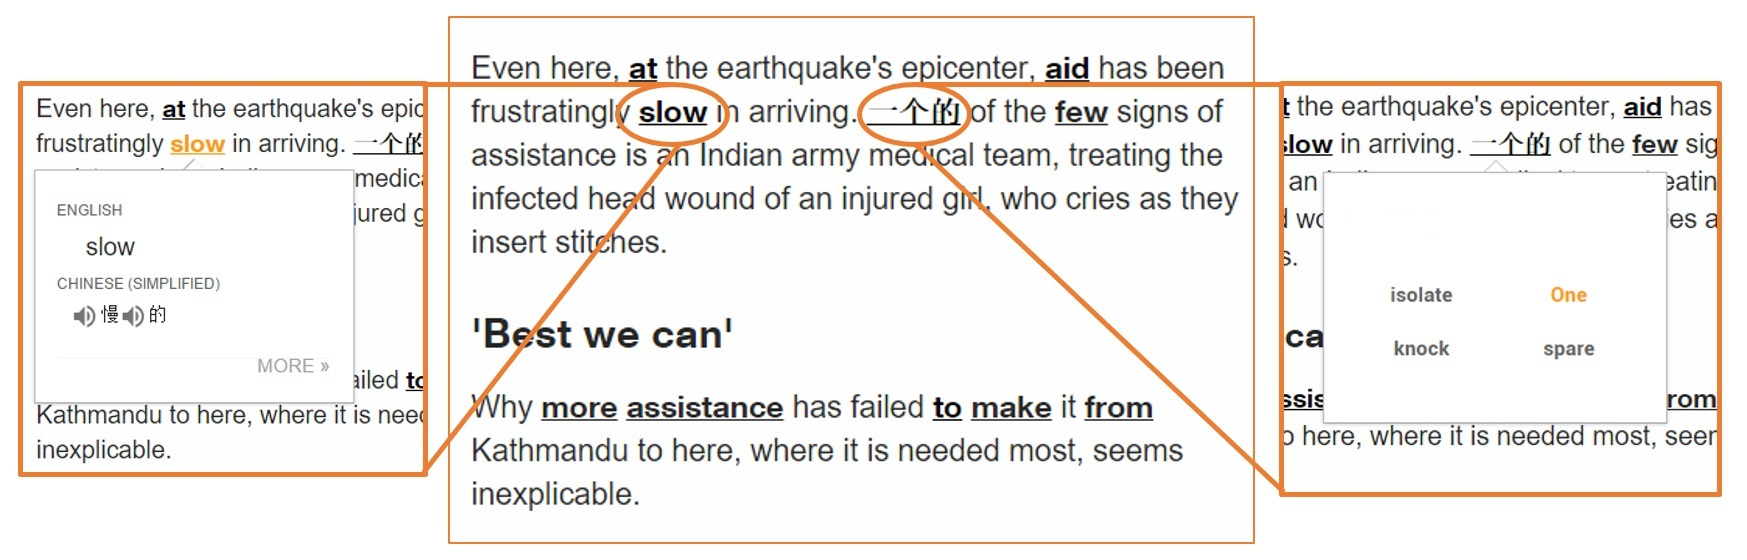
\includegraphics[width=0.99\textwidth]{chrome_extension.jpg}
\caption{Merged screenshots of our Chrome extension on the CNN English
  article {\it Treacherous journey to epicenter of deadly Nepal
    earthquake}.  Underlined components are clickable to yield
  tooltips of two different forms: (l) a definition for learning, (r)
  a multiple-choice interactive test.}
\label{fig:chrome_extension_1}
\end{figure*}

\section{The {\tt SystemA} Chrome Extension}
%%Muthu: To introduce and motivate context here
% Tao: Please mention our bilinguial dictionary 


We give a running scenario to illustrate the use of our language
learning platform, {\tt SystemA}.  When a learner browses to an
English webpage on a news website, our extension selectively replaces
certain original English words words with their Chinese translation
(Figure~\ref{fig:chrome_extension_1}, middle).  While the meaning of
the Chinese word is often apparent in context, the learner can choose
to learn more about the replaced word, by mousing over the translation
to reveal a definition tooltip (Figure~\ref{fig:chrome_extension_1},
left) to aid mastery of the Chinese word.  Once the learner has
encountered the replaced word a few times, {\tt SystemA} will assess
the learner's mastery by generating a multipl choice translation test
on the target word (Figure~\ref{fig:chrome_extension_1}, right).  Our
learning platform thus can be viewed as have three logical components:
{\it translating}, {\it learning} and {\it testing}. \\

%% \begin{figure}[ht]
%%   \centering
%%   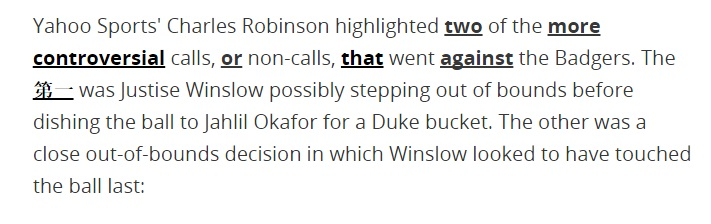
\includegraphics[width=0.45\textwidth]{software_design_2.jpg}
%%   \caption{Screen shot of Translating Component}
%%   \label{fig:software_design_2}
%% \end{figure}
{\bf Translating.}  We pass the main content of the webpage from the
extension client to our server for candidate selection and
translation.  As certain words are polysemous, the server must select
the most appropriate translation among all possible meanings.  Our
initial selection method replaces any instance of words stored in our
dictionary.  For translation, we check the word's stored meanings
against the machine translation of each sentence obtained from the
Microsoft Bing Translation API (hereafter, ``Bing'').  Matches are
deemed as correct translations and are pushed back to the Chrome
client for rendering.

%% \begin{figure}[ht]
%%   \centering
%%     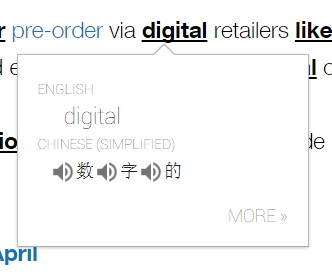
\includegraphics[width=0.3\textwidth]{software_design_4.jpg}
%%   \caption{Screen shot of popover with highlighted English word}
%%   \label{fig:software_design_4}
%% \end{figure}
%%  \begin{figure}[ht]
%%      \centering
%%     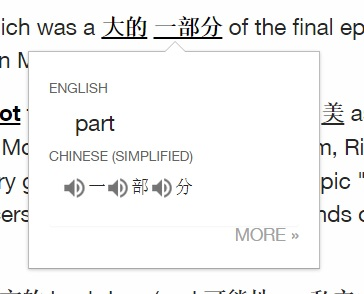
\includegraphics[width=0.3\textwidth]{software_design_5.jpg}
%%      \caption{Screen shot of popover with highlighted Chinese word}
%%      \label{fig:software_design_5}
%%  \end{figure}

{\bf Learning.} Hovering the mouse over the replacement Chinese word
causes a tooltip to appear, which gives the translation,
pronunciation, simplified and traditional written form, and a {\tt
  More} link that loads additional contextual example sentences (that
were previously translated by the backend) for the learner to study.
The more link must be clicked for activation, as we find this
two-click architecture helps to minimize latency and the loading of
unnecessary data.  The server keeps record of the learning tooltip
activations, logging the enclosing webpage URL, the target word and
the user identity.
% Min: doesn't seem to be shown, actually.  Where is an example sentence?
%  Figure \ref{fig:software_design_5} is the screen
% shot of the pop over with its example sentences.

%% \begin{figure}[ht]
%% \centering
%%   \centering
%%   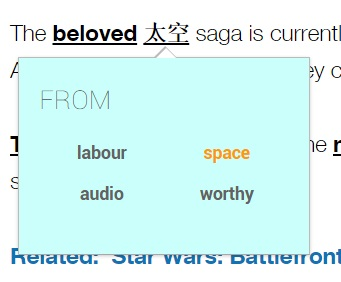
\includegraphics[width=0.3\textwidth]{software_design_7.jpg}
%%   \caption{Screenshot of English test popover}
%%   \label{fig:software_design_7}
%% \end{figure}
%% \begin{figure}[ht]
%%     \centering
%%   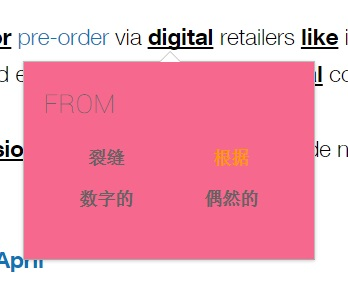
\includegraphics[width=0.3\textwidth]{software_design_8.jpg}
%%   \caption{Screen shot of Chinese test popover}
%%   \label{fig:software_design_8}
%% \end{figure}

{\bf Testing.}  After the learner encounters the same word a
pre-defined number $t=$BUG times, {\tt SystemA} generates a MCQ test
to assess mastery.  When the learner hovers over the replaced word,
the test is shown for the learner to select the correct answer. When
an option is clicked, the server logs the selection, and the correct
answer is revealed by the client extension.  Statistics on the user's
test history are also updated.

%{\bf Classifying words category.}
% Tao: please keep the label, as I have referred it in wsd section
% Min: will note and change
\subsection{News Categories}
\label{subsec:category}

As our learning platform is active only on certain news websites, we
model the news category of both individual words and webpages.  Of
particular import to {\tt SystemA} is the association of words to a
news category, which is used downstream in both word sense
disambiguation (Section~\ref{sec:wsd}) and the generation of
distractors in the interactive tests (Section~\ref{sec:distractor}.
Here, our goal is to automatically find highly relevant words to a
particular news category -- e.g., ``what are typical {\it finance}
words?''.  

We first obtain a large sample of categorized English news webpages,
by creating custom crawlers for specific news websites.  We use a seed
list of words that are matched against a target webpage's URL.  If any
match, the webpage is deemed to be of that category.  For example, a
webpage that has the seed word ``football'' in its URL is deemed of
category ``Sports''.  After a survey of a number of news websites, we
decided on seven categories: namely, ``World'', ``Technology”,
“Sports”, “Entertainment'', ``Finance'', ``Health'' and
``Travel''.  

We tokenize and part-of-speech tag the main body text of the
categorized articles, discarding punctuation and stopwords.  The
remaining words are classified to a news category based on document
frequency.  A word $w$ is classified to a category $c$ if it appears a
tunable threshold $\delta=$BUG more often than its average category
document frequency.  Note that a word can be categorized to multiple
categories under this scheme.

%% A word w is classified into category C(i) if it satisfies Equation~\ref{equation:Distractor_3}::

%% \begin{equation}
%% f (w, C(i)) - sw(w)/n >= \delta
%% \label{equation:Distractor_3} 
%% \end{equation}  

%% The confidence factor $\delta$ can be a positive integer between 0 and the average number of articles in each category. It means on average, the word w must appear in a specific category C(i) $\delta$ times more than it appear in other category before it can be classified into category C(i).

%% It is obvious that a higher confidence factor value will result in less number words getting classified, but it will result in getting words that are more accurate. A suitable confident value is selected to generating category-related words in the later section.






\section{Word Sense Disambiguation System}
\begin{CJK}{UTF8}{gbsn}
As we all know, one word may have multiple translations in another language, and our extension is expected to select the most appropriate one based on the context.We call such translation selection as cross-lingual word sense disambiguation (WSD).

In this following, I describe four approaches that I have tried to accomplish WSD system, which is also my main progress in the second semester. The four approaches are: 

\begin{itemize}
\item Frequency based: always selecting the most frequent translation (the baseline),
\item Part-of-Speech Tag based: selecting the translation based on the Part-of-Speech Tag of the English word
\item Translation based: Selecting the translation based on the result from existing Machine Translation systems
\item Category based: Selecting the translation based on the category of the news article
\end{itemize}

\begin{table*}[t]
  \caption{Example input/output of WSD}
  \label{table:wsd_1}
  \begin{center}
  \begin{tabular}{| p{3cm} | p{1cm} | p{3.5cm} | p{1.2cm} | p{1.3cm}| p{0.8cm} | p{0.9cm} | p{1cm} |}
    \hline
    English Sentence & Word & Dictionary & Baseline & Category & Bing & Bing+ & Bing++ \\
    \hline
    ... treating me like family ... & like & \parbox[t]{3cm}{verb : 喜欢, 爱...\\ ... \\preposition : 好像, 好比 ...} & 喜欢 & 好像 & & & \\
    \hline
    ... painting a picture of urban street life ... & picture & \parbox[t]{3cm}{... 相, 影, 影片(entertainment), 帧, 想象, 画 ...} & & 影片 & & & \\
    \hline
    ... pistol a pump shotgun ... & pump & \parbox[t]{3cm}{verb:抽, 抽水, 打气, 唧, 唧筒, 套\\ noun:抽水机, 唧筒} & & & 唧筒 & & \\
    \hline
    ... have made it into the worlds top 40 clubs ... & top & \parbox[t]{3cm}{顶部, 顶端, 顶, 颠, 盖, 极 ...} & 顶部 &  & 顶 & 顶级 & \\
    \hline
    state department spokeswoman ... & state & \parbox[t]{3cm}{...陈, 陈说, 称, 称述, 发表, 发言...} & & & 发言 & 发言人 & 国家 \\
    \hline
    ...  ... &  & \parbox[t]{3cm}{...  ...} & & & & & \\
    \hline
  \end{tabular}
  \end{center}
\end{table*}

\subsection{Baseline}
The simplest way to select a translation from the candidates is by random. However, the correctness of this method is very low, probably less than 20\%, and is not a good baseline for other methods to compete with. Another simple idea is to always select the most commonly used translation. Luckily, when I crawled the dictionary, Google Translate does provide usage frequency of each Chinese Translation.  This turns out to be a much better result, and thus serves as a fair baseline method.

\subsection{Part-of-Speech Tagger}
As we all know, many English words have more than one Part-of-Speech (POS) tags and their Chinese translations in different POS may differ a lot. For example, the word ``book" has two POS tags, noun and verb. If it is used as a noun, mostly it means a handwritten or printed work of fiction or nonfiction, which should be translated as \begin{CJK}{UTF8}{gbsn}``书"\end{CJK}, and mostly means to reserve if used as a verb, which should be translated as \begin{CJK}{UTF8}{gbsn}``预定"\end{CJK}. Therefore, getting the POS tag of the English word might help us identify its sense or the Chinese translation. We decide use Stanford Log-linear Part-of-Speech Tagger \cite{Toutanova2003}.

Firstly, if the word "like" need to be translated, the algorithm will fetch all the Chinese translations as well as their Part-of-Speech tag from our dictionary. Secondly, the algorithm will send the original English sentence to Part-of-Speech Tagger, which is a Java package and has been wrapped into a server. After the client has got the output from the server, it will fetch the corresponding tag and match it to Part-of-Speech tag based on the guidelines mentioned above. Lastly, it will select the translations based on the POS.

\subsection{News Category}
The word ``interest" have two very different translations when it is used as a noun. One translation is about ``the feeling of a person whose attention, concern, or curiosity is particularly engaged by something", which should be translated as ``兴趣". The other translation is about ``a share, right, or title in the ownership of property", which should be translated as ``利息". It is quite obvious that the second sense is mostly used in financial related topics. Therefore, analysing the category of the original article and selecting the translation with the same category label might help disambiguate the word meaning.

In Table~\ref{table:wsd_1}, word ``picture" is the word that need to be translated. Firstly, the algorithm will fetch all the Chinese translations for word ``picture" and only the word ``影片" has a category ``entertainment". Next, the algorithm will fetch the category of the English news article from the URL, which is also ``entertainment".In this case, the algorithm will use ``影片" as the translation for word ``picture". If a few words shares the same category, the algorithm will choose the translation with the highest frequency of use.

\subsection{Machine Translation}
Since our target is to select the most appropriate translation based on the context, using existing Machine Translation (MT) systems is also a good approach, as all of them will certainly translate words based on the context. After I tried a few on-line or off-line MT systems, We decide to use Bing Translator as our Machine Translation system.

\subsubsection{Bing}

In the example, the original English sentence is ``including a 45-caliber pistol a pump shotgun and an ar-15 rifle" and ``pump" is the word that we want to translate. Firstly, this algorithm will fetch all the Chinese translations from the database. Next, it will send the original English sentence to Bing Translator using the API provided by Microsoft and get the result that returned from Bing Translator. After that, for each Chinese translation, I will check whether this translation is a substring of the Bing Translator result. If there are a few translations that can match with the Bing Translator result, I will select the longest translation. If there are a few translations with the same length and all of them can match with the Bing Translator result, I will select the translation with the highest frequency of use. In this example, both ``唧" and ``唧筒" are the substrings of Bing Translator result. As ``唧筒" have two characters and ``唧" only have one character, this algorithm will take ``唧筒" as the final result.

\subsubsection{Bing+}
 is the approach of using Bing Translator together with Stanford Word Segmenter, and I would like to use Bing+ to represent this algorithm. Step one, two and three has been described in the previous section as it is exactly the same as Bing approach. From Bing approach, this algorithm will generate ``顶" as the result. After that, Bing+ approach will send the Chinese sentence returned from Bing Translator to Stanford Word Segmenter. Then, this algorithm will use the segmented word that contains the Bing result as a substring or equals to the Bing result as the final result. In this example, the final result of Bing+ is ``顶级" which is the best result that can be generated from the result of Bing Translator and also a result that does not covered by our dictionary.

\subsubsection{Bing++}
The Bing++ algorithm is basically the approach of using Bing+ approach together with the Microsoft Bing Word Alignment. First few steps are exactly the same as Bing+ approach. In this example, ``state" is the word that need to be translated. The result from Bing+ approach is ``发言人", which is the translation of ``spokeswoman", because the Chinese translation ``发言" can be translated from both ``state" and ``spokeswoman". Then step five will send the original English sentence to Bing Word Alignment. Now, there will be two final results, one from Bing+ approach and the other one from Bing Word Alignment and the algorithm will choose the correct one from these two results. In this example, ``state" will match with ``国家" and the algorithm will choose ``国家" as the final result as well.

\subsection{WSD System}
Our Word Sense Disambiguate System can be evaluated from two important aspects: coverage (i.e., is able to return a translation) and accuracy (i.e., the translation is proper). To this end, I manually annotate the ground truth.

\begin{table}[ht]
  \caption{Coverage for different approaches}
  \label{table:evaluation_1}
  \begin{tabular}{| p{2cm} | p{2cm} | p{2cm} |}
    \hline
     & Coverage & Accuracy\\
    \hline
    Baseline & 100\% & 57.3\%\\
    \hline
    POSTagger & 94.5\% & 55.2\%\\
    \hline
    News Category & 2.0\% & 7.1\%\\
    \hline
    Bing & 78.5\% & 79.8\%\\
    \hline
    Bing+ & 75.7\% & 80.9\%\\
    \hline
    Bing++ & 76.9\% & 97.4\%\\
    \hline
  \end{tabular}
\end{table}

Table~\ref{table:evaluation_1} column two contains the coverage for different approaches. As the algorithm will try to translate some word only if it is covered by our dictionary, the coverage for Baseline is always 100\%. The coverage for Bing, Bing+, Bing++ and POSTagger are roughly the same and all of them are acceptable. However, the coverage for News Category approach is only 2.0\%. One reason is that when I set the threshold for assigning categories for Chinese word, I purposely make it very high to maximize the accuracy. If the accuracy is quite high, which means this approach is quite useful, then I will lower the threshold and find the balance point.

Figure~\ref{table:evaluation_1} column three contains the accuracy of all the approaches. The last column is the accuracy for News Category approach and it is only 7.1\%. As mentioned in above Chapter, since the accuracy is very low, there is no need to lower the threshold and try to allocate more categories for Chinese words. The accuracy for Baseline is 57.3\%, which is already a fairly hight accuracy. The accuracy for  POSTagger is around 55.2\% also, which is a bit lower than our expectation. The accuracy for Bing++ is 97.4\% which I think is a very good result and it is already very hard to improve. Therefore, based on my test results, Bing++ is the best approach among these five approaches.

\end{CJK}
\section{Distractors Generation Algorithm}
\label{sec:distractor}
Vocabulary testing is a key functionality in our extension. In this section, we investigate a way to automatically generate suitable distractors (in English form) for a target word. We postulate "a  set of suitable distractors" as: 1) being the same form as the target word, 2) fitting the reading context,  and 3)
having proper difficulty level according to user's knowledge skill.

By applying Part-of-Speech tagger, we obtain the POS tag for the target word, and then restrict the  candidate distractors to be selected from the same word class.
To make the distractors fitting the context, we identify news category  (approach is detailed in Section~\ref{subsec:category}), and select the distractors from the same category.



%To generate good category-related distractors, it is essential to gather enough words that are more related in a certain category to serve as distractors candidates. By using the approach discussed in Section~\ref{subsec:category}, we crawled more than 1400 articles for seven categories, with around 200 articles in each category. The confidence factor is selected to be 10, which is suitable to classify enough words into different categories. After this step, there should be sufficient “Category-Related" words in each category.


The difficulty of a distractor is measured by its {\bf semantic distance} to the target word: a closer is,  a more difficult distractor is. To quantify the semantic distance, we employ  Lin Distance~\cite{lin98}  to measure the distance betwen two words in WordNet~\cite{Miller1995} and define  distractors to be difficult if the Lin Distance score is below some threshold.
By observing the generated distractors, we empirically set $0.1$ as the threshold.

%The selection of threshold value will have a direct effect on the speed of distractors generation process. As a very high threshold value will result in more rounds of calculation in semantic distance calculator, and it will take a long time before the distractors are returned to the front end. After several rounds of analysis of each category’s words and the results returned from semantic distance calculator, the threshold value of 0.1 is selected.





%{\bf Semantic Distance.}
%Before we go to explain the next step, it is essential to introduce the semantic distance calculator we used in the server implementation. 
%
%The perspective of semantic relatedness or its inverse, semantic distance, is a concept that indicates the likeness of two words. It is more general than the concept of similarity as stated in WordNet’s synset relation. Similar entities in WordNet are classified into same synset based on their similarity. However, dissimilar entries may also have a close semantic connection by lexical relationships  such as meronymy (car-wheel) and antonymy (hot-cold), or just by any kind of functional relationship or frequent association(pencil-paper, penguin-Antarctica) \cite{ale01}. Semantic distance calculator aims to calculate the semantic relatedness score between two words.
%
%There are many approaches to calculate semantic relatedness score. In this application, we are using Lin Distance \cite{lin98} to calculate the semantic distance between two concepts. The detail of Lin Distance methodology is explained as follows.
%
%Lin attempted to define a measure of semantic similarity that would be both universal and theoretically justified. There are three intuitions that he used as a basis:
%\begin{itemize}
%\item The similarity between arbitrary objects A and B is related to their commonality; the more commonality they share, the more similar they are;
%\item The similarity between A and B is related to the differences between them; the more differences they have, the less similar they are.
%\item The maximum similarity between A and B is reached when A and B are identical, no matter how much commonality they share. 
%\end{itemize}
%
%Based on the intuition above, Lin proposed his approach in measuring similarity between two concepts c1, c2 in Equation~\ref{equation:Distractor_4}:
%
%\begin{equation}
%sim(c1,c2) = \frac{2*log_p(lso(c1,c2))}{log_p(c1)+log_p(c2)}
%\label{equation:Distractor_4}
%\end{equation}  
%
%where p(c) denotes the probability of encountering concept c, and lso(c1,c2) denotes the lowest common subsumer, which is the lowest node in WordNet hierarchy that is a hypernym of c1 and c2. 
%
%The distance calculator will return a score from 0 to 1, as can be easily seen from the formula above. If the score is closer to 1, it means the two words are closer in semantic sense. This distance calculator will play an important role in the following algorithm. 

%\subsubsection{Distractors Selection Algorithm}
\subsection{User knowledge Aware Approach}
As mentioned, our extension logs user's detailed learning history, and we categorize user's knowledge  on a certain word into three levels, based on the number of times that he/she has encountered  the word.  Then we adopt different strategies to generate  distractors for users in different knowledge level. 

% Tao: please fill the BUG by the actual number and quantify "just learnt" etc.
% Zhao: Filled already.

{\bf Knowledge Level 1 (K1)}: This indicated user is tested on this word for the first time. Considering this, our system prefers to generate simple distractors, and thus randomly select three words from the same news category. 

{\bf Knowledge Level 2 (K2)}: This indicates that the user has known this word for three times. Therefore, the testing is expected to be harder. Our system first randomly selects two words from the same news category. For the third distractor,  the system keeps randomly selecting distractor from the same category, computing its semantic distance to the target word, and stops until meeting a difficulty one.


{\bf Knowledge Level 3 (K3)}: This indicates that the user already has a good understanding of the word, {\it i.e.}, passing the test for six times. As such, we make the test even harder, and choose  three difficulty distractors from the new category. 

%; the algorithm will choose distractors solely based on results returned from semantic distance calculator. Similar to the approach when knowledge level is 2, the algorithm will randomly select word from current category’s word list and calculate the semantic distance between the selected word and the target word. If the score is above certain threshold, the selected word is chosen as one of the distractors. The process is continued until the server can find three distractors. 


\subsection{Evaluation}
% Tao: How to choose the third distractor? from d2's 
% Zhao: The three distractors are all selected from the same synset.
To compare with our proposed method, we further implemented an existing distractor generation method  used in WordGap system~\cite{Knoop2013}. WordGap still adopts knowledge-based approach, selecting the synonyms of synonyms (computed in WordNet) as the distractors. That is, we select the most frequently used word (referred as w1), from the target word’s synonym set. %Then we select the synset, let's call it  s1, which the synset where the most frequently used word of w1 lies in. 
Then we select the synonyms of w1 and call this set as s1.
Synset s1 contain all the words that are synonyms of synonyms of the target word. Finally we select three most frequently used words from s1 as distractors for the baseline approach.

For our proposed method, we adopt three different strategies to generate distractors, according to user's knowledge level. In our evaluation, we focus on assessing distractors generated for two extreme cases, {\it i.e.}, knowledge level 1, and knowledge level 2. Therefore, we conduct a pairwise comparison -- K1  vs. Baseline, and K3  vs. Baseline, using the same testing dataset.



%There are two evaluations to be done as follows:
%1.  Compare Baseline with Knowledge Level 1 Algorithm
%
%.  Compare Baseline with Knowledge Level 3 Algorithm
%For each comparison, three distractors are generated from the baseline algorithm; three distractors are generated from the stated algorithm in this report. With the first comparison we will be able to see if the category information will help in selecting more suitable distractors. By comparing the results from the both evaluation, we will be able to see if semantic distance and category information will help improve the suitability of distractors.

%he first distractor {\textit d1} is the most frequently used word from target word’s synonym set, and the second distractor {\textit d2} is the most frequently used synonym for  {\textit d1},
%similarly, {\textit d3} BUG (HOW TO GENERATE d3). However, if the number of valid result we can get is less than three, we will choose the word that shares the same antonym with the target word.

%To evaluate the distractors selection strategy as described in this report, we chose the knowledge-based approach used by many other language learning systems, which is to utilize the WordNet data and selection distractors based on synonyms of synonyms. WordGap system uses this approach to generate vocabulary test for its android application.

%In our implementation of the baseline algorithm, we will choose the most frequent used word w1 from the target word’s synonym set, and select the most frequent used word w2 from word w1’s synonym set. The selection process is continued until we can find 3 distractors to form a vocabulary test. However, if the number of valid result we can get is less than 3, we will choose the word that shares the same antonym with the target word.


\subsubsection{User Study}
To compare the two approaches in generating distractors, we turn to users, asking users to compare the plausibility of distractors.
%To compare the two approaches in generating distractors, we designed several survey sets to ask users to compare the plausibility of distractors.
 We randomly selected 50 sentences from recent news articles and then chose a noun or adjective from the sentence as the target word. In our survey, each question looks like a real MCQ quiz: we show the original sentence (leaving the target word as blank) as the context,  and randomly display the six distractors and the target word as choices. Users are required to read the sentence and select the correct answer (that they think) as rating 1, and 
 rank the other choices from 2 (most plausible) to 7 (least plausible) based on their plausibility. Figure~\ref{fig:distractor_1} shows an example survey question.
 
 %In the survey, participants are required to answer each question and rank the plausibility of all distractors from 1 to 7. The correct answer will be ranked as 1, and the least plausible distractor will be ranked as 7. A screenshot of one sample question is shown in Figure \ref{fig:distractor_1}.

We have two tests (K1  vs. Baseline, and K3  vs. Baseline) and each contains 50 questions. We further group 25 questions as one session, and give users the freedom to participate one or more sessions. Each question will be answered by at least five different users.
Finally, we recruited 15 users from our university, and half of them are native English speakers. 
% Tao: please check
%In average, each user participate two sessions.



%The evaluation contains 100 questions and is separated into 4 surveys, with each survey containing 25 questions. Each participant is free to choose one or more than one surveys. The purpose is to reduce the workload in each survey to get better responses. The surveys are sent to Year 1 students from School of Computing, National University of Singapore.  There are 15 valid responses with each participant ranking each distractor with a different weight from 1 to 7. Half of the participants are native English speakers.



\begin{figure}[ht]
   \centering
   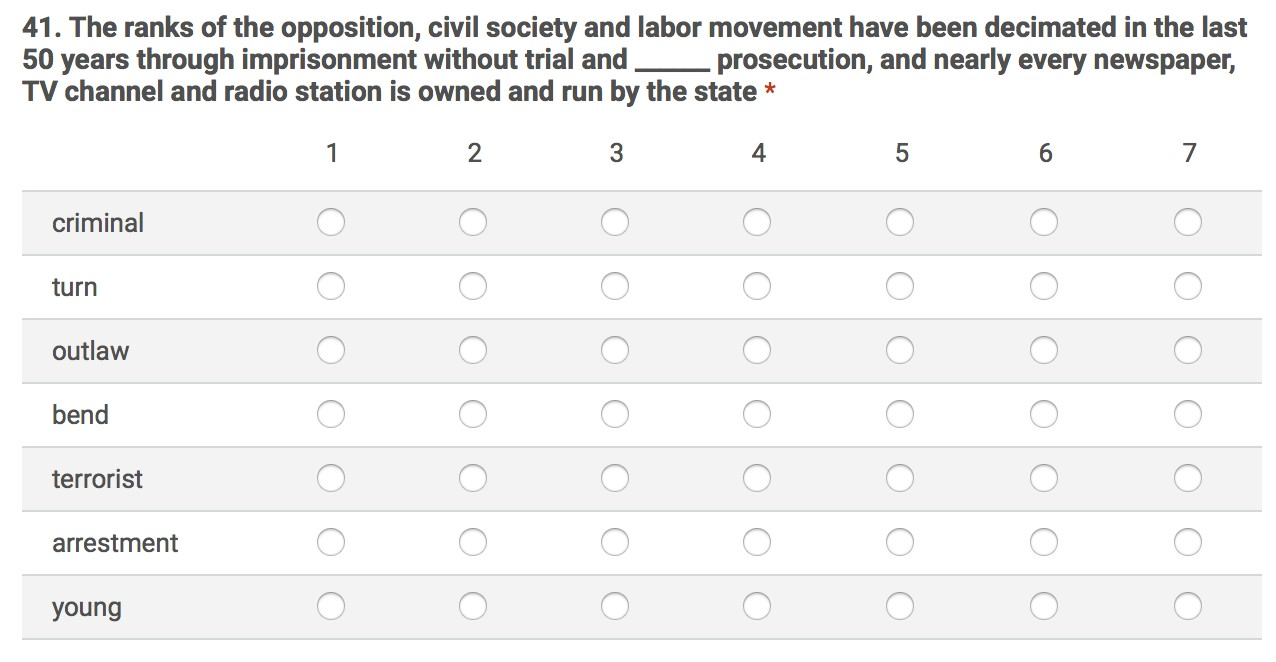
\includegraphics[width=0.45\textwidth]{distractor_1.jpg}
   \caption{A sample survey question}
   \label{fig:distractor_1}
\end{figure}

\subsubsection{Results}
As each question is answered by five different users, we compute the average rating for each choice. A lower rating means a more plausible (harder) distractor. 
% Tao: Plese fill 
Unsurprisingly, the rating for all the target words is low ($1.1$ in average), as they are the ground truth. This implies that the users answered the survey questions seriously, and the evaluation quality is controlled.


%Each participant’s rank will be the weight of the particular distractor in that question, i.e. if the user rank one distractor as rank “5”, the weight of this distractor in this user’s response will be 5. For each distractor of each question, the ranks of all users’ responses are summed. As the more plausible the distractor is, the higher rank it will have, thus if the sum is higher, the approach is not as plausible as the other from user’s point of view.

\begin{table}[ht]
    \caption{ Resutls: Baseline vs. Knowledge Level 1 Algorithm}
    \label{table:distractor_1}
    \begin{center}
    \begin{tabular}{| p{1.5cm} | p{2.5cm} | p{2.2cm} |}
        \hline
         & Number of winning questions & Average score\\
        \hline
        Baseline & 27 & 3.84\\
        \hline
        K1 & 23 & 4.10\\
        \hline
    \end{tabular}
    \end{center}
\end{table}

\begin{table}[ht]
    \caption{Results: Baseline vs. Knowledge Level 3 Algorithm}
    \label{table:distractor_2}
    \begin{center}
    \begin{tabular}{| p{1.5cm} | p{2.5cm} | p{2.2cm} |}
        \hline
         & Number of winning questions & Average score\\
        \hline
        Baseline & 21 & 4.16\\
        \hline
        K3 & 29 & 3.49\\
        \hline
    \end{tabular}
    \end{center}
\end{table}

Table \ref{table:distractor_1} and Table \ref{table:distractor_2} showed the detailed result of each comparison. If for any question, the sum of weight from all participants for one approach is bigger than the other, then this approach is considered to have won this question. The “average score” is the average sum of weight from each approach for all questions. The lower the average score is, the better performance this approach has gained.

From Figure \ref{fig:distractor_1} we can see that in the first comparison, the baseline algorithm actually outscored the knowledge level 1 generation algorithm by 4 questions, with a sum of weight lower than 0.26. From Table \ref{table:distractor_1} we can see that in the second comparison, the knowledge level 3 generation algorithm surpassed the baseline algorithm by 8 questions, with the average weight of 3.49 vs 4.16. 

\subsubsection{Analysis}
In knowledge level 1 generation algorithm, there is no semantic distance calculation involved. If the target word to test has no strong category indication, for example, words like 'venue', 'week', it is possible that the knowledge level 1 algorithm will select some distractors that are not as plausible as those coming from the target word's synonym of synonym. 

However, this problem is solved with the help of semantic distance calculator. In the knowledge level 3 generation algorithm, the distractors chosen are both semantic close and also category-related, which produced a relatively better experiment result.

Also in the baseline algorithm, it is possible that it will select words that are very rare in real life \cite{sus13}, which may also have influence in the result.

\section{Evaluation}





\section{Conclusion}
\label{sec:conclusion}

We described WordNews, a client extension and server backend that
transforms the web browser into a second language learning platform.
Leveraging web-based machine translation APIs and a static dictionary,
it offers a viable user-driven language learning experience by pairing
an improved, context-sensitive tooltip definition service with the
generation of context-sensitive multiple choice questions.

WordNews is potentially not confined to use in news websites; one
respondent noted that they would like to use it on arbitrary websites,
but currently we feel usable word sense disambiguation is difficult
enough even in the restricted news domain.  We also note that
respondents are more willing to use a mobile client for news reading,
such that our future development work may be geared towards an
independent mobile application, rather than a browser extension.  We
also plan to conduct a longitudinal study with a cohort of second
language learners to better evaluate WordNews' real-world effectiveness.



% include your own bib file like this:
%\bibliographystyle{acl}
%\bibliography{acl2015}
% use socreport.bst
\bibliographystyle{acl}
\bibliography{acl2015}

%\clearpage\end{CJK*}
\end{document}
